%==============================================================

\section{Big Data Framework Spark}\label{bds1}

After all features are extracted, the next step is to load the feature files into the HDFS.
All feature files of the same type (forming the feature sets) get merged into one large file. For the about 114000 songs all feature files sum up to about 11.2 GB (see figure \ref{filesize}). 

\begin{figure}[htbp]
	\centering
	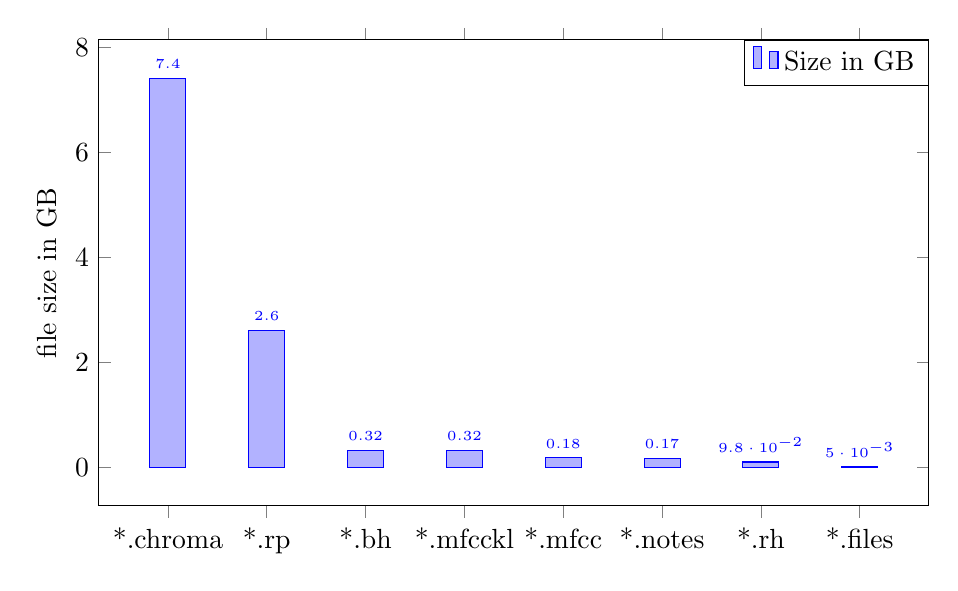
\begin{tikzpicture}
		\begin{axis}[
		    width=\textwidth,height=75mm,% <- added
		    x tick label style={/pgf/number format/1000 sep=},
      		xticklabels={ ,  , *.chroma, *.rp, *.bh, *.mfcckl, *.mfcc, *.notes, *.rh, *.files}, 
		    ylabel=file size in GB,
		    %enlargelimits=0.05,% <- commented, default is .1
		    legend style={
		      at={(1,1)},
		      anchor=north east,% <- changed
		      %legend columns=-1% <- commented
		    },
		    nodes near coords,
		    every node near coord/.append style={font=\tiny},
		    %nodes near coords align={vertical},% <- commented, default
		    ybar=0pt,%<- changed
		    bar width=13pt% <- added
		  ]
		  \addplot
		    coordinates {(1,7.400) (2,2.600) (3,0.324) (4,0.324) (5,0.177) (6,0.174) (7,0.098) (8,0.005)};
		  \legend{Size in GB}
		\end{axis}
	\end{tikzpicture}
	\caption{File sizes}
	\label{filesize}
\end{figure}

\noindent Large streaming platforms like Spotify give access to about 30 million songs in their databases. At this scale, the feature files would approximately sum up to about 3 TB.\\

\subsection{Underlying hardware}

The first tests with Spark were performed on a single PC with 4 CPU cores (8 with HT) (Intel Core i7-3610QM CPU, 2.30GHz × 4) running Spark 2.4.0.\\ The cluster test were performed on the ARA-cluster, that offers 16 compute-nodes with 32 CPU-cores (Dual Socket, 2 x Intel Xeon "Scalable" 6140, 2.30 GHz x 18) per node (72 with HT) and 192GB of RAM. The cluster was running an older version of Spark (1.6.0)\\

\subsection{Workflow}

Although multiple different implementations were tested to evaluate the fastest and most efficient way to compute the similarities, all of these different approaches follow the same basic steps. These can be seen in figure \ref{workflowspark}.  

\begin{figure}[htbp]
	\centering
	\framebox{\parbox{1\textwidth}{ 	
		\centering
		\ \\
		%\smartdiagramset{set color list={blue!40!white, blue!40!white,blue!40!white, blue!40!white, blue!40!white, blue!40!white}}
		\tikzset{priority arrow/.append style={rotate=180,anchor=0,xshift=30,}}			
		\smartdiagram[priority descriptive diagram]{5) return result, 4) joining results, 3) distance scaling, 2) distance computation, 1) data preparation and caching} \\
		\caption{Workflow Spark}
		\label{workflowspark}
	}}
\end{figure}
\FloatBarrier

\noindent The following sections explain the various stages in more detail, also giving more details over a few subtle differences between the different implemented and tested approaches like the usage of RDDs, single DataFrames for each feature or one large DataFrame containing all features. 

\subsection{Data preparation}

The features are stored in text files as described in chapter \ref{sumfeat}. Due to the fact that the features were extracted in parallel and in batches of only a few songs, each of the feature files only contain the features of a small number of songs. Because many small files are inefficient to process with Spark \cite[p. 153]{sparkbook1} all files containing the same feature type are merged to one large file, before being loaded into the HDFS. By loading larger files into the HDFS, the partitioning into data blocks is performed according to the standard parameters of the HDFS (e.g. 128 MB partitions). Additional repartitioning on the cluster is later performed with Spark by using the \lstinline{rdd.repartition(repartition\_count)} command. 
Finally to work with the features a few transformations have to be performed on the data. For example the extracted note values are stored as lists of integer numbers, each representing a certain note. To compare these using the Levenshtein distance, these lists are converted into strings. 

\begin{pythonCode}[frame=single,label={lst:prep1},caption={notes preprocessing},captionpos=b]
chroma = sc.textFile("features/out[0-9]*.notes").repartition(repartition_count)
chroma = chroma.map(lambda x: x.split(';'))
chroma = chroma.map(lambda x: (x[0], x[1], x[2], x[3].replace("0",'A').replace("1",'B').replace("2",'C').replace("3",'D').replace("4",'E').replace("5",'F').replace("6",'G').replace("7",'H').replace("8",'I').replace("9",'J').replace("10",'K').replace("11",'L'))).map(lambda x: (x[0], x[1], x[2], x[3].replace(',','').replace(' ','')))
df = spark.createDataFrame(chroma, ["id", "key", "scale", "notes"])
\end{pythonCode}

\noindent All the other features are stored as lists of floats and have to be converted to vectors. The Spark ML library and the older MLlib library offer sparse and dense vectors as a data type. The only feature type that contains a lot of zeros and where sparse vectors could improve performance is the beat histogram. But compared to other features like the chromagram they are relatively small (with a length of only 200 values) so all lists including the beat histograms are converted to dense vectors by calling \lstinline{Vectors.dense(l)}. An example is given for the rhythm pattern features in code snippet \ref{lst:rpp}.

\begin{pythonCode}[frame=single,label={lst:rpp},caption={rp preprocessing},captionpos=b]
from pyspark.mllib.linalg import Vectors
list_to_vector_udf = udf(lambda l: Vectors.dense(l), VectorUDT())
rp = sc.textFile("features[0-9]*/out[0-9]*.rp").repartition(repartition_count)
rp = rp.map(lambda x: x.split(","))
kv_rp = rp.map(lambda x: (x[0].replace(";","").replace(".","").replace(",","").replace(" ",""), list(x[1:])))
rp_df = spark.createDataFrame(kv_rp, ["id", "rp"])
rp_df = rp_df.select(rp_df["id"],list_to_vector_udf(rp_df["rp"]).alias("rp"))
\end{pythonCode}

\noindent The data is read out of the HDFS into an RDD and repartitioned with \lstinline{sc.textFile("name.txt")}. The repartitioning is optional but improves the overall performance (see \ref{sparkperf}). After the pre-processing steps are performed the RDD can be converted into a Spark SQL DataFrame by calling \lstinline{spark.createDataFrame()} to ease up the access to the data and improve the code readability. The features can then be accesses via column names instead of the RDD indices, making the code better readable and understandable.\\
For the performance tests three different kind of implementations were tested. The first one merges all audio features into one large DataFrame in the beginning and persists this to the main memory. The second implementation uses single DataFrames for each feature set and the third uses RDDs instead of DataFrames. The results of the performance analysis of DataFrames vs. RDDs are given in section \ref{sparkperf}

\subsection{Distance Computation}

After the data preparation, the similarities between a requested single song and all other songs in the database can be calculated. The code differs slightly when using RDDs instead of DataFrames. The full source code is attended in the appendices on the included CD and can be checked out from github \cite{github-code}. Most of the following code examples were written for the usage with DataFrames. The examples for the usage with RDDs are annoted accordingly.\\

\subsubsection{Euclidean Distance}

The euclidean distance is used as a metric to compute the distances between the vectors of beat histograms, rhythm histograms, rhythm patterns and MFCCs making it the most versatile distance measurement introduced in this thesis. To compute the euclidean distance in Spark a user defined function (UDF) is declared (see \ref{lst:eucd}). This UDF is then applied to all elements of the \lstinline{'features'} column. Inside the UDF the euclidean distance is computed using python's scipy library. Alternatively the numpy library could be used as well (\lstinline{numpy.linalg.norm(x-comparator_value)}). 

\begin{pythonCode}[frame=single,label={lst:eucd},caption={euclidean distance DF},captionpos=b]
from scipy.spatial import distance
from pyspark.sql import functions as F
distance_udf = F.udf(lambda x: float(distance.euclidean(x, comparator_value)), FloatType())
result = feature_vec_df.withColumn('distances', distance_udf(F.col('features')))
result = result.select("id", "distances").orderBy('distances', ascending=True)
result = result.rdd.flatMap(list).collect()
\end{pythonCode}

\noindent The \lstinline{comparator_value} variable contains the feature of the requested example song to which the distances are calculated. Assuming that all features were merged into one large DataFrame (\lstinline{fullFeatureDF}) and cached to the main memory, the \lstinline{comparator_value} can be found by filtering the DataFrame for the requested songs ID (e.g. the path name of the original song).

\begin{pythonCode}[frame=single,label={lst:comp},caption={Filter for requested song},captionpos=b]
song = fullFeatureDF.filter(fullFeatureDF.id == songname).collect()
comparator_value = song[0]["mfccEuc"]
\end{pythonCode}

\noindent When working with RDDs instead of DataFrames, the computation of the distances between the feature vectors is performed with a \lstinline{map()} instead of a UDF (see code snippet \ref{lst:eucr}). 

\begin{pythonCode}[frame=single,label={lst:eucr},caption={euclidean distance RDD},captionpos=b]
resultRP = rp_vec.map(lambda x: (x[0], distance.euclidean(np.array(x[1]), np.array(comparator_value))))
\end{pythonCode}

\subsubsection{Bucketed Random Projection}

As an alternative to the euclidean UDF, Spark offers an implementation of a Locality-sensitive hashing (LSH) family for the euclidean distance called Bucketed Random Projection. The Spark API documentation describes the idea behind LSH as stated: "The general idea of LSH is to use a family of functions (“LSH families”) to hash data points into buckets, so that the data points which are close to each other are in the same buckets with high probability, while data points that are far away from each other are very likely in different buckets." \cite{lshspark} The BRP projects the feature vectors $x$ onto a random unit vector $v$ and portions the projected result into hash buckets with the bucket-length $r$. "A larger bucket length (i.e., fewer buckets) increases the probability of features being hashed to the same bucket (increasing the numbers of true and false positives)." \cite{lshspark}

\begin{equation} \label{eq:brp}
h(x) = \left \lfloor{\frac{x \cdot v}{r}}\right \rfloor 
\end{equation}

\noindent The method \lstinline{model.approxNearestNeighbors(dfA, key, k)} searches for the \lstinline{k} nearest neighbors of \lstinline{dfA} to the \lstinline{key} but the Spark API documentation mentions that "Approximate nearest neighbor search will return fewer than k rows when there are not enough candidates in the hash bucket." \cite{lshspark}
This means that the smaller (and therefor more precise) the bucket length is, the fewer nearest neighbors get returned by this function. This is problematic when searching for the nearest neighbors of different features sets because the resulting distances calculated from the different kind of features have to be joined to get the resulting similarities as a combination of different distance measurements (see section \ref{weighedsum}). If the BRP only returns a handful of nearest neighbors, the overall distances to all the other songs can not be determined.\\
\noindent Due to the fact that the ARA-cluster is running with PySpark version 1.6.0 and the Bucketed Random Projection (BRP) was introduced with PySpark version 2.2.0, the algorithm could only be tested on the single node test platform where it performed worse than the naive euclidean implementation from code snippet \ref{lst:eucd} on a dataset consisting of about 11500 songs. Whether the BRP outperforms the naive approach on a cluster with bigger datasets could be investigated further. 

\begin{pythonCode}[frame=single,label={lst:brp},caption={bucketed random projection},captionpos=b]
from pyspark.ml.feature import BucketedRandomProjectionLSH
#...
brp = BucketedRandomProjectionLSH(inputCol="features", outputCol="hashes", seed=12345, bucketLength=100.0)
model = brp.fit(feature_vec_df)
comparator_value = Vectors.dense(comparator[0])
result = model.approxNearestNeighbors(feature_vec_df, comparator_value, feature_vec_df.count()).collect()
rf = spark.createDataFrame(result)
result = rf.select("id", "distCol").rdd.flatMap(list).collect()
\end{pythonCode}

 

\subsubsection{Cross-correlation}

As laid out in chapter \ref{melsimc} there are different options to calculate the cross-correlation of the beat-aligned chroma features. The chroma features are allready key-shifted to a common key but the possibility to perform a full 2D-cross-correlation with additional key-shifting as explained in equation \ref{eq:conv2}, \ref{eq:conv3} and \ref{eq:conv4} still exists. But due to the fact that the computation of the cross-correlation already takes the most time even without additional key-shifting (see section \ref{sparkperf}) the implementation on the cluster and in code snippet \ref{lst:corrnp} calculates the simplified cross-correlation (equations \ref{eq:conv5} and \ref{eq:conv6}). Whether or not the results are compromised because of that is left open and requires further investigation.\\
\noindent The cross-correlation was used to detect cover songs on the same dataset Ellis and Cotton used in their paper\cite{cover802}. The results are presented in chapter \ref{covsongid}. There are some differences in the results to the original paper. These can be explained with the different underlying beat tracking, different filter parameters and a few improvements that are left out compared to the implementation of Ellis \cite{cover802} as mentioned in \ref{chromafeat}.\\
Concerning the actual implementation of the cross-correlation, two different libraries were tested. Code snippet \ref{lst:corrsc} shows the cross-correlation function coming with the scipy library.

\begin{pythonCode}[frame=single,label={lst:corrsc},caption={cross-correlation scipy},captionpos=b]
corr = scipy.signal.correlate2d(chroma1, chroma2, mode='full')
\end{pythonCode}

\noindent The parameter \lstinline{mode='valid'} determines whether or not additional key shifting is included. The \lstinline{'valid'} option already includes additional key-shifting but without zero-padding. Other options would be \lstinline{mode='same'}(no key-shifting) and \lstinline{mode='full'} (with zero-padding)\\
\noindent The other variant is shown in code snippet \ref{lst:corrnp}. It uses the numpy library. Although numpy only offers a 1D-cross-correlation function which had to be nested inside a for-loop to get the 2D-cross-correlation, but performance tests showed that the numpy version was faster than the scipy version by orders of magnitude. Calculating and scaling the distances of the chroma features from one song to about 114000 other songs took about 22 seconds with numpy and around 725 seconds with scipy on the ARA-cluster. 

\begin{pythonCode}[frame=single,label={lst:corrnp},caption={cross-correlation numpy},captionpos=b]
from scipy.signal import butter, lfilter, freqz, correlate2d, sosfilt
import numpy as np
def cross_correlate(chroma1, chroma2):
    length1 = chroma1_par.size/12
    chroma1 = np.empty([12, length1])
    length2 = chroma2_par.size/12
    chroma2 = np.empty([12, length2])
    if(length1 > length2):
        chroma1 = chroma1_par.reshape(12, length1)
        chroma2 = chroma2_par.reshape(12, length2)
    else:
        chroma2 = chroma1_par.reshape(12, length1)
        chroma1 = chroma2_par.reshape(12, length2)      
    correlation = np.zeros([max(length1, length2)])
    for i in range(12):
        correlation = correlation + np.correlate(chroma1[i], chroma2[i], "same")    
    #remove offset to get rid of initial filter peak (highpass filter jump 0-20)
    correlation = correlation - correlation[0]
    sos = butter(1, 0.1, 'high', analog=False, output='sos')
    correlation = sosfilt(sos, correlation)[:]
    return np.max(correlation)
#...
distance_udf = F.udf(lambda x: float(cross_correlate(x, comparator_value)), DoubleType())
result = df_vec.withColumn('distances', distance_udf(F.col('chroma')))
result = result.select("id", "distances").orderBy('distances', ascending=False)
result = result.rdd.flatMap(list).collect()
\end{pythonCode}

\subsubsection{Jensen-Shannon-like Divergence}

While computing the Jensen-Shannon-like Divergence for the MFCC features a problem with negative determinants was encountered. Because the logarithm of negative numbers is not defined, no similarity for these features could be calculated.\\ 
Schnitzer mentioned a problem with "skyrocketing values of determinants which lead to inaccurate results" \cite[p.45]{schnitzer1}. He proposed a solution by using the sum of the upper triangular matrix of the Cholesky decomposition to compute the logarithm of the determinant of the covariance matrix in equation \ref{eq:jsl3}. 
This approach was also tested for the encountered issue mentioned above but ultimately did not work out because of the covariance matrices not being positive definite.\\
Because no immediate solution to that problem was found, the rows where this issue appears just get filtered out by setting the distance to \lstinline{np.inf} and later dropping these rows. This problem seems to appear for about 5-10\% of the distances calculated with the Jensen-Shannon Divergence. Further investigation to solve this problem would be necessary. 
An example code snippet is given in \ref{lst:js}.

\begin{pythonCode}[frame=single,label={lst:js},caption={Jensen-Shannon-like Divergence},captionpos=b]
import numpy as np
def jensen_shannon(vec1, vec2):
	#preprocessing: splitting vec1 and vec2 into mean1, mean2, cov1 and cov2
	mean_m = 0.5 * (mean1 + mean2)
	cov_m = 0.5 * (cov1 + mean1 * np.transpose(mean1)) + 0.5 * 
		(cov2 + mean2 * np.transpose(mean2)) - (mean_m * np.transpose(mean_m))
	div = 0.5 * np.log(np.linalg.det(cov_m)) - 0.25 * np.log(np.linalg.det(cov1)) - 
		0.25 * np.log(np.linalg.det(cov2))  
	if np.isnan(div):
		div = np.inf
	return div
distance_udf = F.udf(lambda x: float(jensen_shannon(x, comparator_value)), 
	DoubleType())
result = df_vec.withColumn('distances', distance_udf(F.col('features')))
result = result.filter(result.distances_js != np.inf)    
result = result.select("id", "distances").orderBy('distances', ascending=True)
result = result.rdd.flatMap(list).collect()
\end{pythonCode}

\subsubsection{Symmetric Kullback-Leibler Divergence}\label{sparkskl}

When implementing the Symmetric Kullback-Leibler Divergence a few interesting observations could be made. First of all this metric seems to be prone to outliers. While only very few distances get disproportionately large, most of the distances are between 0 and 100. The large outliers lead to problems when scaling the resulting distances to an interval between 0 and 1 (see section \ref{distsc} and \ref{featqual}). As a temporary solution all distances larger than a certain threshold get filtered out.\\ 
Secondly when using the fma dataset a few of the songs returned error where the covariance matrix could not be inverted. 
These songs get filtered out as well. The example code for the calculation of distance using DataFrames can be seen in code snippet \ref{lst:kl}. 

\begin{pythonCode}[frame=single,label={lst:kl},caption={Kullback-Leibler Divergence},captionpos=b]
import numpy as np
def symmetric_kullback_leibler(vec1, vec2):
	#preprocessing: splitting vec1 and vec2 into mean1, mean2, cov1 and cov2
	if (is_invertible(cov1) and is_invertible(cov2)):
		d = 13
		div = 0.25 * (np.trace(cov1 * np.linalg.inv(cov2)) + 
			np.trace(cov2 * np.linalg.inv(cov1)) + 
			np.trace((np.linalg.inv(cov1) + 
			np.linalg.inv(cov2)) * (mean1 - mean2)**2) - 2*d)
	else: 
		div = np.inf
		#print("ERROR: NON INVERTIBLE SINGULAR COVARIANCE MATRIX\n")  
	return div
distance_udf = F.udf(lambda x: float(symmetric_kullback_leibler(x, comparator_value)), DoubleType())
result = df_vec.withColumn('distances', distance_udf(F.col('features')))
#thresholding for outliers
result = result.filter(result.distances <= 100)  
#result = result.filter(result.distances != np.inf)        
result = result.select("id", "distances").orderBy('distances', ascending=True)
result = result.rdd.flatMap(list).collect()
\end{pythonCode}

\noindent After implementing this similarity measurement into Spark some tests and comparisons to the results of the musly toolkit \cite{musly1} were done. While overall the genre recall is quite good (see chapter \ref{genrerec}) and the results are reasonable they do differ from the ones returned from musly. 
These differences in the results to the original musly tool could be explained with to the choice of only 13 MFCC bands in this thesis compared to the 25 bands in musly \cite{musly1} and some other decisions like leaving the normalization with mutual proximity (\ref{mprox}) out. The same goes for the Jensen-Shannon-like Divergence. 


\subsubsection{Levenshtein distance}

Spark already offers a function for the computation of the Levenshtein distance when the feature vectors are stored in a DataFrame. The Levenshtein distance can then be computed between two columns for all rows. Code snippet \ref{lst:levd} shows a minimal example. 

\begin{pythonCode}[frame=single,label={lst:levd},caption={Levenshtein DataFrame},captionpos=b]
from pyspark.sql.functions import levenshtein 
df_merged = featureDF.withColumn("compare", lit(comparator_value)) 
df_levenshtein = df_merged.withColumn("word1_word2_levenshtein", levenshtein(col("notes"), col("compare")))
df_levenshtein.sort(col("word1_word2_levenshtein").asc()).show()
\end{pythonCode}

\noindent An alternative for the RDD based variant of the Spark application the python wrapper for the C/C++ library edlib was used. During initial tests when experimenting with an naive implementation of the levenshtein distance using a python function with numpy immense performance issues were encountered. Due to the underlying C/C++ code of the edlib the computation of the levenshtein distance in code snippet \ref{lst:levr} performes comparably well as the Spark-native DataFrame equivalent and is a good alternative. 

\begin{pythonCode}[frame=single,label={lst:levr},caption={Levenshtein RDD},captionpos=b]
import edlib
def naive_levenshtein(seq1, seq2):
    result = edlib.align(seq1, seq2)
    return(result["editDistance"])
#...
resultNotes = notes.map(lambda x: (x[0], naive_levenshtein(str(x[1]), str(comparator_value)), x[1], x[2]))
\end{pythonCode}

\subsubsection{Lazy evaluation and caching data}\label{leval}

As described in chapter \ref{sparksec} Sparks main advantage is its ability to use the main memory of the nodes in a cluster to safe intermediate data without the need of writing it back to the disk. However Spark does not automatically cache the data. RDDs and DataFrames have to be explicitly assigned to the RAM by either calling \lstinline{persist()} (optionally with the parameter \lstinline{storageLevel=StorageLevel.MEMORY_ONLY_SER}) or \lstinline{cache()} and even then Spark only takes this function only as a suggestion. If not enough main memory is available, the data is still written onto the hard drives. As introduced in chapter \ref{sparksec} Spark uses an optimization technique called lazy evaluation that differentiates between transformations on data and actions. The \lstinline{cache()} and \lstinline{persist()} commands both do not count as actions. Instead they are executed only when an actual action on the data is called. This have to be kept in mind when optimizing Spark applications and evaluating the performance by measuring execution times. The code snippet \ref{lst:persist} gives a short example. 

\begin{pythonCode}[frame=single,label={lst:persist},caption={Spark lazy evaluation},captionpos=b]
import time
#...
featureDf = preprocess_features().persist()	#p3
print(featureDf.first()) #p4
tic1 = int(round(time.time() * 1000))
neighbors = get_distances(songname, featureDf).persist() #p6
neighbors = neighbors.orderBy('scaled_dist', ascending=True).persist() #p7
neighbors.show()
neighbors.toPandas().to_csv("neighbors.csv", encoding='utf-8')
neighbors.unpersist()
tac1 = int(round(time.time() * 1000))
time_dict['time: ']= tac1 - tic1
print time_dict
\end{pythonCode}

\noindent \lstinline{preprocess_features()} is a function where the chroma features get read into RDDs, pre-processed, repartitioned and converted to a DataFrame.\lstinline{get_distances()} calculates all distances between the song belonging to the ID \lstinline{songname} and the other 114209 songs in the database. Within this function the results are then scaled to an interval between 0 and 1 by dividing all distances by the maximum distance. The result is stored in the DataFrame \lstinline{neighbors} and after that two actions are performed subsequently on this result. The first (\lstinline{show()}) prints the 20 nearest neighbors to the standard output. The second action (\lstinline{toPandas().to_csv()}) prints the whole list of all 114210 distances into a *.csv file.\\
In a simple experiment the impact of ineffective caching and the impact of the lazy evaluation on time and performance tests is shown. The results are plotted in figure \ref{lazcach}. The first bar shows the \lstinline{print time_dict} output when executing the full code from code sample \ref{lst:persist}. In the second bar labeled with "p6" the \lstinline{persist()} command in line 6 got removed. Due to the fact that the scaling of the distances inside the function \lstinline{get_distances()} requires an action on the data but the results are no longer persistent in the cache, this part of the code has to be executed twice. For the third bar labeled with "p7", the \lstinline{persist()} command in line 7 is removed as well. The result \lstinline{neighbors} is no longer stored in the main memory and every time an action requires this DataFrame, it has to be recalculated which is the case for both actions in line 8 and line 9 of the code example.\\
When further removing the print command in line 4, the lazy execution no longer executes line 3 before starting to measure the time in line 5 because the action \lstinline{first()} is no longer executed on the DataFrame. Instead line 3 gets called when calling \lstinline{get_distances()} because only then an action on the featureDf DataFrame is called for the first time. This is shown in the bar labeled with "l4". Up until this point the original featureDf still gets persisted to the main memory but if the \lstinline{persist()} command in line 3 gets removed as well in the last test labeled with "p3" the \lstinline{preprocess_features()} has to be executed every time \lstinline{get_distances()} is called.  

\begin{figure}[htbp]
	\centering
	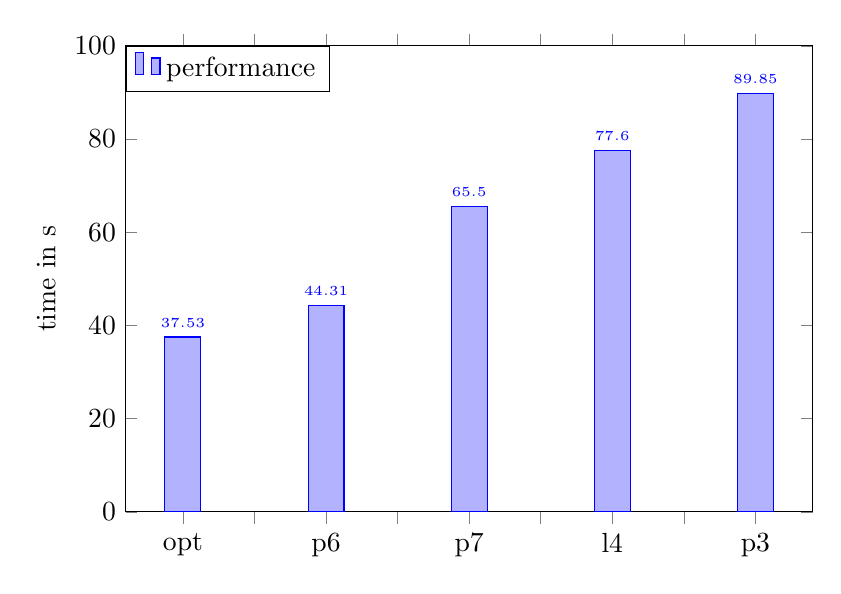
\begin{tikzpicture}
		\begin{axis}[
				width=0.85\textwidth,height=75mm,% <- added
				x tick label style={/pgf/number format/1000 sep=},
				xticklabels={ ,  , opt, , p6, , p7, , l4, ,p3}, 
				ylabel=time in s,
				ymin=0, ymax=100,
				%enlargelimits=0.05,% <- commented, default is .1
				legend style={
				at={(0,1)},
				anchor=north west,% <- changed
				%legend columns=-1% <- commented
				},
				nodes near coords,
				every node near coord/.append style={font=\tiny},
				%nodes near coords align={vertical},% <- commented, default
				ybar=0pt,%<- changed
				bar width=13pt% <- added
				]
			\addplot
				coordinates {(01,37.527) (02,44.310) (03,65.495) (04,77.597) (05,89.846)};
			\legend{performance}
		\end{axis}
	\end{tikzpicture}
	\caption{Lazy evaluation and caching}
	\label{lazcach}
\end{figure}
\FloatBarrier

\noindent So in summary the correct way of caching data is a tricky task. Writing everything into the main memory is no solution either because then the cluster will run out of memory eventually. As a rule of thumb the best way to persist data is to cache it every time more than one subsequent action is performed on it.\\
For the field of music similarity hat means that especially all pre-processed features have to fit into the main memory of the cluster to speed up consecutive song requests. 

\subsection{distance scaling}\label{distsc}

To combine different distance measurements into one combined distance the various results from the different kind of features have to be rescaled to avoid biasing the overall distance.
The easiest way is to subtract the minimum of all distances $d$ and dividing by the difference between the maximum and the minimum distance as described in equation \ref{eq:scaling}. 

\begin{equation} \label{eq:scaling}
d' = \frac{d - min(d)}{max(d) - min(d)}
\end{equation}

\noindent The minimum distance should always be the self-similarity of the requested song with a value of 0 but in the implementation the Symmetric Kullback-Leibler distance this isn't always the case. The analysis of the distances in chapter \ref{featqual} also shows that e.g. the levenshtein distances and cross-correlation results are unequally distributed over the interval between 0 and 1 (unit interval $[0,1]$). Dropping the self-similarity out of the distance vector and rescaling it afterwards with a new miniumum distance unequal to zero could solve this but was not tested in this thesis. A second issue was already mentioned in section \ref{sparkskl} where outliers tend to bias the results. These can get filtered out before rescaling the distances. This is further evaluated in chapter \ref{featqual}.\\
Another option to rescale the features laid out by Sebastian Stober in \cite[pp. 543ff]{musicdata} but not implemented in this thesis would be to rescale all distances to have a mean value of 1 by using equation \ref{eq:scaling2} by dividing the distance by the mean distance $\mu_f$. Outliers should be detected and removed before calculating the mean distance. 
A better way to rescale the data could be evaluated in future research. 

\begin{equation} \label{eq:scaling2}
d' = \frac{d}{\mu_f}
\end{equation} 

Implementation-wise the aggregation of the minimum and maximum value went through different tests. During first tests the aggregation of minimum and maximum value were performed separately (see \ref{lst:mindf}). This turned out to be very inefficient because the data had to be accessed multiple times. 

\begin{pythonCode}[frame=single,label={lst:mindf},caption={Minimum and maximum aggregation separate},captionpos=b]
max_val = result.agg({"distances": "max"}).collect()[0]
max_val = max_val["max(distances)"]
min_val = result.agg({"distances": "min"}).collect()[0]
min_val = min_val["min(distances)"]
\end{pythonCode}

An improved version shown in code example \ref{lst:mindf} only uses one action to gather minimum and maximum value, which improved the overall performance significantly. 

\begin{pythonCode}[frame=single,label={lst:mindf},caption={Minimum and maximum aggregation optimized},captionpos=b]
from pyspark.sql import functions as F
aggregated = result.agg(F.min(result.distances),F.max(result.distances))
max_val = aggregated.collect()[0]["max(distances)"]
min_val = aggregated.collect()[0]["min(distances)"]
\end{pythonCode}

Another alternative would be the usage the \lstinline{describe()} function for DataFrames. For the implementation using RDDs the \lstinline{stats()} function was used, returning minimum, maximum, mean and variance values all at once. 

\subsection{Combining different measurements}\label{weighedsum}

To finally compute the overall similarity of what Stober calls the facet distances in \cite[pp. 543ff]{musicdata} (the different distances computed using different feature sets) the weighted arithmetic mean of the previously scaled facet distances is calculated by using equation \ref{eq:distance}.

\begin{equation} \label{eq:distance}
dist = \frac{\sum_{m = 0}^{M - 1}{w_m \cdot d_m}}{\sum_{m = 0}^{M - 1}{w_m}}
\end{equation}

In this thesis only binary weights were tested by either including a facet distance with a weight of one or just leaving it out of the overall similarity by setting its weight to zero. The impact of different weights is left open for future research. 

\subsection{performance}\label{sparkperf}

\subsubsection{Cluster configuration} %and data file size}

The first thing that had to be done was to alter the spark cluster configuration for the ARA-cluster as described in chapter \ref{cconfexp}. With the help of the \lstinline{spark.dynamicAllocation} parameters the amount of Executors spawned can be determined. While normally the executors are spawned and then retained for the life of the application, dynamicAllocation is able to free the resources of Executors that are idle for a long time and to reassign the belonging system resources.\\
The cluster configuration in the code example \ref{lst:clust} turned out to perform best. The cluster is configured in a way where 16 up to 32 Executors are spawned with each Executor requesting as many CPU cores and memory resources as possible. 
The \lstinline{repartition_count} variable is used with the \lstinline{repartition()} method during the data preparation stage to evenly distribute all chunks of feature file across the cluster. 

\begin{pythonCode}[frame=single,label={lst:clust},caption={cluster setup},captionpos=b]
confCluster = SparkConf().setAppName("MusicSimilarity Cluster")
confCluster.set("spark.driver.memory", "64g")
confCluster.set("spark.executor.memory", "64g")
confCluster.set("spark.driver.memoryOverhead", "32g")
confCluster.set("spark.executor.memoryOverhead", "32g")
#confCluster.set("yarn.nodemanager.resource.memory-mb", "196608")
confCluster.set("spark.yarn.executor.memoryOverhead", "4096")
confCluster.set("spark.driver.cores", "32")
confCluster.set("spark.executor.cores", "32")
confCluster.set("spark.dynamicAllocation.enabled", "True")
confCluster.set("spark.dynamicAllocation.minExecutors", "16")
confCluster.set("spark.dynamicAllocation.maxExecutors", "32")
confCluster.set("yarn.nodemanager.vmem-check-enabled", "false")
repartition_count = 32
\end{pythonCode}

\noindent To get the most performant cluster configuration various cluster settings were tested. 
Increasing the \lstinline{repartition_count} and the amount of Executors spawned (with fewer ressources each) seemingly only increased the overhead and network traffic on the cluster without reducing the overall computation time. Only increasing the \lstinline{repartition_count} while keeping the Executors as large as in the code snippet turned out to be slower as well.\\ 
Although each node on the ARA-cluster has 36 CPU cores (without hyper-threading), 32 cores assigned to each Executor turned out to perform just a little bit better when calculating the similarities for only one song in the first tests. Therefor the cluster configuration was set as described in the code snippet \ref{lst:clust} for the following tests in this section.\\
When calculating the similarities on already cached feature data for consecutive song requests, 36 cores per executor performed slightly better than 32 cores. Increasing the CPU core count to 72 per Executor performed far worse.\\

%\noindent FMA Many Small Files (40000 small files, 102000 songs)\\
%MFCC + NOTES + RP:      {'TOTAL DF': 30517, 'TOTAL RDD': 211591, 'TOTAL MERGED': 39336}\\
%JS + CHROMA + RP:       {'TOTAL DF': 32439, 'TOTAL RDD': 130989, 'TOTAL MERGED': 41490}\\                               
%FMA ONE large file / feat (8 larger files, 102000 songs)\\
%MFCC + NOTES + RP:      {'TOTAL DF': 33677, 'TOTAL RDD': 21933, 'TOTAL MERGED': 31963}\\
%JS + CHROMA + RP:       {'TOTAL DF': 41477, 'TOTAL RDD': 35856, 'TOTAL MERGED': 51286}    
                                    
\subsubsection{Differences between the feature types}

Due to the different complexity of the various similarity measurements and metrics, the time needed to calculate the distances between all songs and a single requested song differs. The computation time of all feature types (with respect to the lazy evaluation as described in section \ref{leval}) is pictured in figure \ref{features}. 

\begin{figure}[htbp]
	\centering
	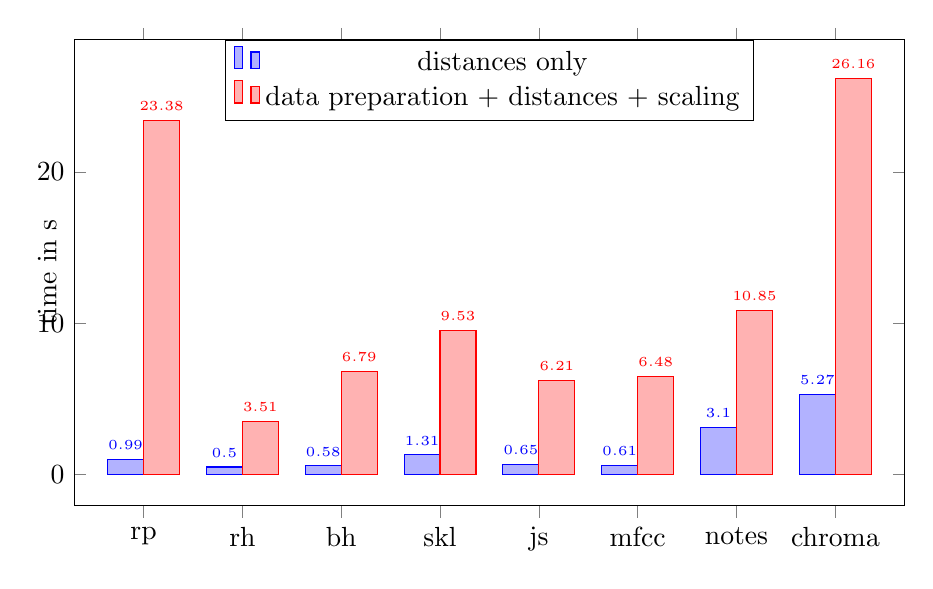
\begin{tikzpicture}
		\begin{axis}[
		    width=\textwidth,height=75mm,% <- added
		    x tick label style={/pgf/number format/1000 sep=0.05},
      		xticklabels={ , ,rp, rh, bh, skl, js, mfcc, notes, chroma}, 
		    ylabel=time in s,
  			y label style={at={(-0.01,0.5)}},
		    %enlargelimits=0.05,% <- commented, default is .1
		    legend style={
		      at={(0.5,1)},
		      anchor=north,% <- changed
		      %legend columns=-1% <- commented
		    },
		    nodes near coords,
		    every node near coord/.append style={font=\tiny},
		    %nodes near coords align={vertical},% <- commented, default
		    ybar=0pt,%<- changed
		    bar width=13pt% <- added
		  ]
		  \addplot
		    coordinates {(1,0.987) (2,0.504) (3,0.575) (4,1.306) (5,0.653) (6,0.613) (7,3.100) (8,5.273)};
		  \addplot
		    coordinates {(1,23.378) (2,3.506) (3,6.792) (4,9.527) (5,6.206) (6,6.475) (7,10.846) (8,26.160)};
		  \legend{distances only, data preparation + distances + scaling}
		\end{axis}
	\end{tikzpicture}
	\caption{Performance on different feature types}
	\label{features}
\end{figure}
\FloatBarrier

\noindent The blue bars figure the computation time required to compute the distances between one requested song and all 114210 songs in the dataset without loading the data and without scaling. That means, that the features were stored in the main memory already. The measured times for the whole computation of the similarities for each feature set including the data time taken for pre-processing and the scaling of the results to the unit interval is shown in the red bar. The plot shows the importance of proper caching for fast response times. 
\noindent The labels on the x-axis represent the different distance measurements and are used further throughout this thesis, mainly in different plots. 

\begin{itemize}
	\setlength\itemsep{-0.5em}
	\item bh (beat histogram, euclidean distance)
	\item rh (rhythm histogram, euclidean distance)
	\item notes (notes, levenshtein distance)
	\item rp (rhythm patterns, euclidean)
	\item mfcc (MFCCs, euclidean distance)
	\item js (MFCCs, Jensen-Shannon-like divergence)
	\item skl (MFCCs, symmetric Kullback-Leibler divergence)
	\item chroma (beat aligned chromagram, cross-correlation)
\end{itemize}

\subsubsection{Data representation}

Figure \ref {perfspark2} and \ref{perfspark3} show the performance of three different approaches on the ARA-cluster for different combinations of features (see caption).\\
For the approach annotated with "Merged DF" all features are pre-processed, joined and storeed in one large DataFrame that then gets repartitioned across all nodes and cached. The idea behind this approach is to reduce shuffling operations during the computation of the similarities by bringing all feature types of the same songs to the same compute nodes. The downside of this method is a higher initial workload that has to be tolerated during the pre-processing stage. Once the pre-processing of the features is done the similarities between the songs are computed and the results are stored in new, smaller DataFrames, one for each feature type. Due to the previous joining of the feature data by the song ID, the repartitioning and the caching, distances of the same songs but for different feature types are calculated on the same node in theory, reducing unnecessary shuffling operation during the compute time. The resulting small DataFrames containing the facet distances for one feature set are joined by the song IDs once all similarities are computed. Then the joined results are scaled using only one \lstinline{agg()} call for all feature types (see section \ref{distsc}) and the combined distances are summed up and sorted. Figure \ref{mergeddf} shows the adapted workflow (original see figure \ref{workflowspark}) of this approach \\

\begin{center}
  \sffamily
  \footnotesize
  \begin{tikzpicture}[auto,
    %decision/.style={diamond, draw=black, thick, fill=white,
    %text width=8em, text badly centered,
    %inner sep=1pt, font=\sffamily\small},
    block_center/.style ={rectangle, draw=black, thick, fill=white,
      text width=14em, text centered, minimum height=2em},
    block_assign/.style ={rectangle, draw=black, thick, fill=white,
      text width=22em, text ragged, minimum height=2em, inner sep=6pt},
	line/.style ={draw, thick, -latex', shorten >=0pt}]
    % outlining the flowchart using the PGF/TikZ matrix funtion
    \matrix [column sep=5mm,row sep=3mm] {
      % enrollment - row 1
      \node [block_center] (b1) {data preparation};
      & \node [block_assign] (c1) {many DFs (features)};\\
      % enrollment - row 2
      \node [block_center] (b2) {join and repartition};
      & \node [block_assign] (c2) {single DF (features)};\\
      % enrollment - row 3
      \node [block_center] (b3) {distance computation};
      & \node [block_assign] (c3) {single DF (features) + many DFs (distances)};\\
      % follow-up - row 4
      \node [block_center] (b4) {join results};
      & \node [block_assign] (c4) {single DF (features) + single DF (distances)};\\
      % follow-up - row 5
      \node [block_center] (b5) {scale results \& combine};
      & \node [block_assign] (c5) {single DF (features) + single DF (distances)};\\
      % follow-up - row 6
      \node [block_center] (b6) {sort and return result};
      & \node [block_assign] (c6) {single DF (features)};\\
    };% end matrix
    % connecting nodes with paths
    \begin{scope}[every path/.style=line]
      % paths for enrollemnt rows
      \path (b1) -- (b2);
      \path (b2) -- (b3);
      \path (b3) -- (b4);
      \path (b4) -- (b5);
      \path (b5) -- (b6);
      \path (b1) -- (c1);
      \path (b2) -- (c2);
      \path (b3) -- (c3);
      \path (b4) -- (c4);
      \path (b5) -- (c5);
      \path (b6) -- (c6);
    \end{scope}
  \end{tikzpicture}
  \captionof{figure}{Workflow Merged DF}
  \label{mergeddf}
\end{center}

%The consideration to join the resulting distances with the large cached feature DataFrame was made but this approach would alter the original feature DataFrame, making it necessary to create a copy of the original DataFrame which leads to additional overhead. 
\noindent The second approach annotated with "DF" also uses DataFrames, but stores the different pre-processed feature types in separate smaller DataFrames instead. The third approach doesn't use DataFrames at all and uses single RDDs for the pre-processed features. Each of the times measured include the full workflow including data pre-processing, calculating, scaling and combining the similarities for a single song request. The plots show the time required to compute the similarities for that single requested song for growing datasets starting from 163 (covers80) to 114210 songs (all datasets combined). 
\noindent Unsurprisingly the Merged DF- approach performed relatively poorly compared to the other approaches due to its initial overhead. The next section will make up for this when presenting the performance on the calculation of subsequent song requests on the same features.

\FloatBarrier
\begin{figure}[htbp]
	\centering
	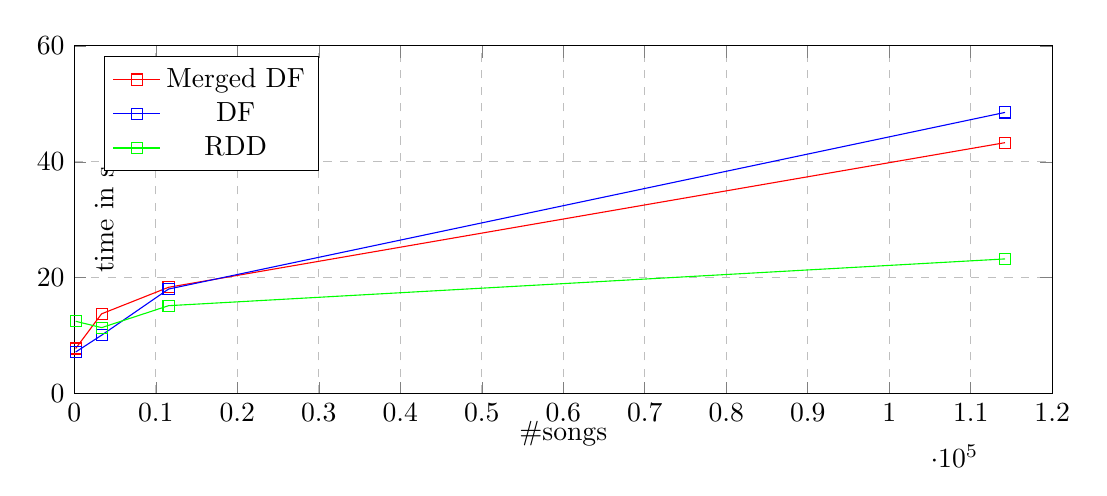
\begin{tikzpicture}
	\centering
	\begin{axis}[
	    %title={Performance of various toolkits},
		x label style={at={(axis description cs:0.5,-0.05)},anchor=north},
		y label style={at={(axis description cs:0.05,.5)},rotate=0,anchor=south},
	    xlabel={\#songs},
	    ylabel={time in s},
	    xmin=0, xmax=120000,
	    ymin=0, ymax=60,
	    %xtick={0,1000,2000,3000,4000,5000,6000,7000,8000,9000,10000,100000,120000},
	    %ytick={0,100,200,300,400,500,600,700,800,900,1000},
	    legend pos=north west,
	    ymajorgrids=true,
	    grid style=dashed,
	    height=6cm,
	    width=14cm,
	    grid=major,
	]
	\addplot[color=red,mark=square,]
		coordinates {(164,7.800)(3344,13.778)(11564,18.356)(114210,43.296)};
		\addlegendentry{Merged DF}		
	\addplot[color=blue,mark=square,]
		coordinates {(164,7.189)(3344,10.090)(11564,18.052)(114210,48.512)};
		\addlegendentry{DF}	
	\addplot[color=green, mark=square,]
	    coordinates {(164,12.490)(3344,11.396)(11564,15.180)(114210,23.245)};
	    \addlegendentry{RDD}	  
	\end{axis}
	\end{tikzpicture}
	\caption{Performance ARA, full workload, (MFCC + Notes + RP)}
	\label{perfspark2}
\end{figure}
\FloatBarrier

\FloatBarrier
\begin{figure}[htbp]
	\centering
	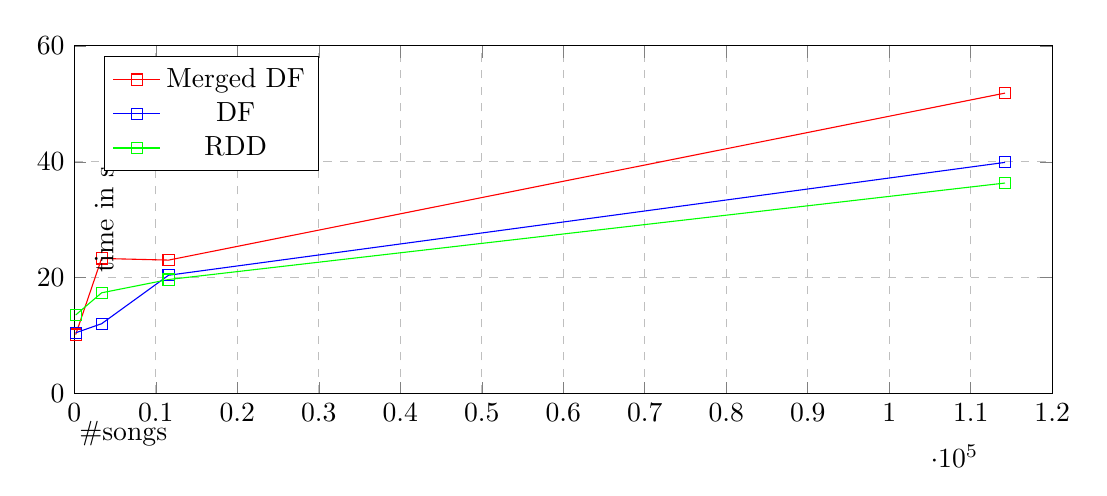
\begin{tikzpicture}
	\centering
	\begin{axis}[
	    %title={Performance of various toolkits},
		x label style={at={(axis description cs:0.05,-0.05)},anchor=north},
		y label style={at={(axis description cs:0.05,.5)},rotate=0,anchor=south},
	    xlabel={\#songs},
	    ylabel={time in s},
	    xmin=0, xmax=120000,
	    ymin=0, ymax=60,
	    %xtick={0,1000,2000,3000,4000,5000,6000,7000,8000,9000,10000,100000,120000},
	    %ytick={0,100,200,300,400,500,600,700,800,900,1000},
	    legend pos=north west,
	    ymajorgrids=true,
	    grid style=dashed,
	    height=6cm,
	    width=14cm,
	    grid=major,
	]
	\addplot[color=red, mark=square,]
		coordinates {(164,10.208)(3344,23.327)(11564,23.042)(114210,51.842)};
		\addlegendentry{Merged DF}	
	\addplot[color=blue,mark=square,]
		coordinates {(164,10.506)(3344,12.069)(11564,20.432)(114210,39.894)};
		\addlegendentry{DF}
   	\addplot[color=green,mark=square,]
		coordinates {(164,13.580)(3344,17.401)(11564,19.692)(114210,36.334)};
		\addlegendentry{RDD}		
	\end{axis}
	\end{tikzpicture}
	\caption{Performance ARA, full workload, (JS + Chroma + RP)}
	\label{perfspark3}
\end{figure}
\FloatBarrier



\subsubsection{Performance for subsequent song requests}

In contrast to the performance analysis from the last section, figure \ref{perfspark4} shows the time measured to process 2 subsequent song requests. That means that the second consecutive song request is able to use the already pre-processed and cached feature data. Figure \ref{perfspark4} shows the according results.\\

\FloatBarrier
\begin{figure}[htbp]
   	\centering
   	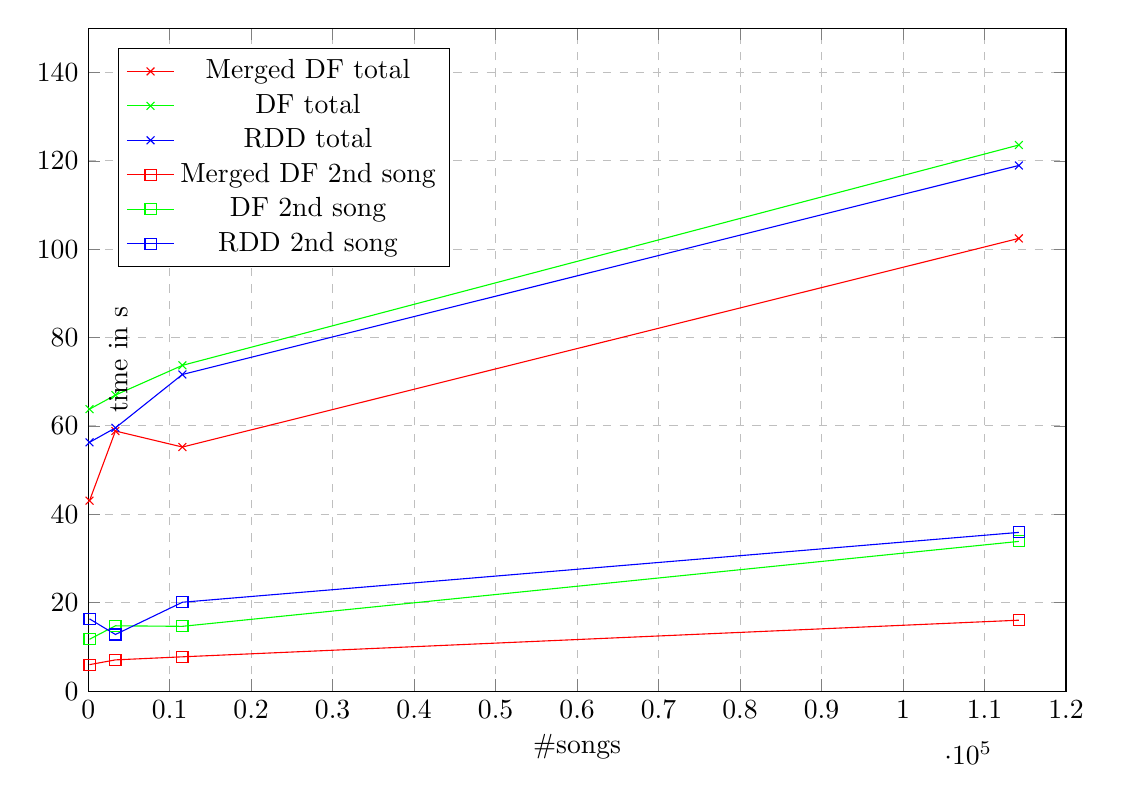
\begin{tikzpicture}
   	\centering
   	\begin{axis}[
	    %title={Performance of various toolkits},
   		x label style={at={(axis description cs:0.5,-0.05)},anchor=north},
   		y label style={at={(axis description cs:0.05,.5)},rotate=0,anchor=south},
	    xlabel={\#songs},
	    ylabel={time in s},
	    xmin=0, xmax=120000,
	    ymin=0, ymax=150,
	    %xtick={0,1000,2000,3000,4000,5000,6000,7000,8000,9000,10000,100000,120000},
	    %ytick={0,100,200,300,400,500,600,700,800,900,1000},
	    legend pos=north west,
	    ymajorgrids=true,
	    grid style=dashed,
	    height=10cm,
	    width=14cm,
	    grid=major,
   	]
   	\addplot[color=red, mark=x,]
   		coordinates {(164,43.090)(3344,58.852)(11564,55.227)(114210,102.438)};
   		\addlegendentry{Merged DF total}
   	\addplot[color=green, mark=x,]
   		coordinates {(164,63.796)(3344,66.986)(11564,73.711)(114210,123.573)};
   		\addlegendentry{DF total}   		
   	\addplot[color=blue, mark=x,]
   		coordinates {(164,56.294)(3344,59.564)(11564,71.648)(114210,118.939)};
   		\addlegendentry{RDD total}   
   				
   	%\addplot[color=red, mark=x, dashed, dotted,]
   		%coordinates {(164,9.043)(3344,14.486)(11564,12.082)(114210,34.781)};
   		%\addlegendentry{Merged DF 1st song}   		
   	%\addplot[color=green, mark=x, dashed,]
   		%coordinates {(164,35.134)(3344,36.699)(11564,42.577)(114210,72.612)};
   		%\addlegendentry{DF 1st song}   		
   	%\addplot[color=blue, mark=x, dashed,]
   		%coordinates {(164,27.233)(3344,34.607)(11564,39.238)(114210,70.488)};
   		%\addlegendentry{RDD 1st song} 
 
   	\addplot[color=red, mark=square, ]
   		coordinates {(164,5.987)(3344,7.063)(11564,7.756)(114210,16.043)};
   		\addlegendentry{Merged DF 2nd song}   		
   	\addplot[color=green, mark=square,]
   		coordinates {(164,11.726)(3344,14.776)(11564,14.655)(114210,33.872)};
   		\addlegendentry{DF 2nd song}   		
   	\addplot[color=blue, mark=square,]
   		coordinates {(164,16.337)(3344,12.809)(11564,20.108)(114210,35.911)};
   		\addlegendentry{RDD 2nd song}   			
   	\end{axis}
   	\end{tikzpicture}
   	\caption{two subsequent songs, all features}
   	\label{perfspark4}
\end{figure}
\FloatBarrier

\noindent The plots annoted with Merge DF total, DF total and RDD total depicture the overall computation time including the pre-processing and the handling of both song requests. The other graphs show the computation time of only the second song request. The measured times include the calculation of the distances, the scaling and the join operation of the different result-types. 
\noindent The results show that the pre-merged DataFrame approach performs best, returning the 20 nearest neighbors for the second song request in about 16 seconds and 14 seconds when using 36 cores per executor as mentioned in section \ref{sparkperf} cluster configuration). 

\subsubsection{Descending importance filter and refine}

To improve the performance even further a filter and refine method was tested where the similarities are computed for one feature set and all songs to which the distance is larger than the mean value of all distances get filtered out of the feature DataFrame. From the thinned-out dataset another less important feature set is chosen and this is repeated until all feature sets were used. 
The implementation is based on the "Merge DF" approach described and pictured in \ref{mergeddf} earlier on but a few changes had to be made. After all features are pre-processed, joined and repartitioned, this large feature DataFrame gets cloned and persisted to the main memory as well. It is important that the compute cluster has enough RAM available to cache the full feature DataFrame twice. 
The first feature set is chosen and the distances are calculated and appended to the cloned version of the full feature DataFrame. 
In the next step all rows of the DataFrame where the freshly calculated distances are larger than some threshold (the mean value of the distance column in this case) get dropped out of the DataFrame, drastically reducing the size of all feature-sets.
When using the mean value about half of the songs get dropped out of the DataFrame, reducing the problem size for the next feature set to half the size. This is also the reason why the data had to be copied in-memory because now the clone can be altered and thinned out without impacting the original DataFrame. Of course the copying of the data on the other hand is an additional overhead. 
But when looking at the results in figure \ref{perfspark5} it shows that the filter and refine method scales very well with increasing sizes of the dataset. The plots show the performance of full requests on already cached feature DataFrames or RDDs but the plots of the filter and refine tests include the time necessary to create a copy of the cached feature DataFrames so the additional overhead is taken into account. 

\FloatBarrier
\begin{figure}[htbp]
   	\centering
   	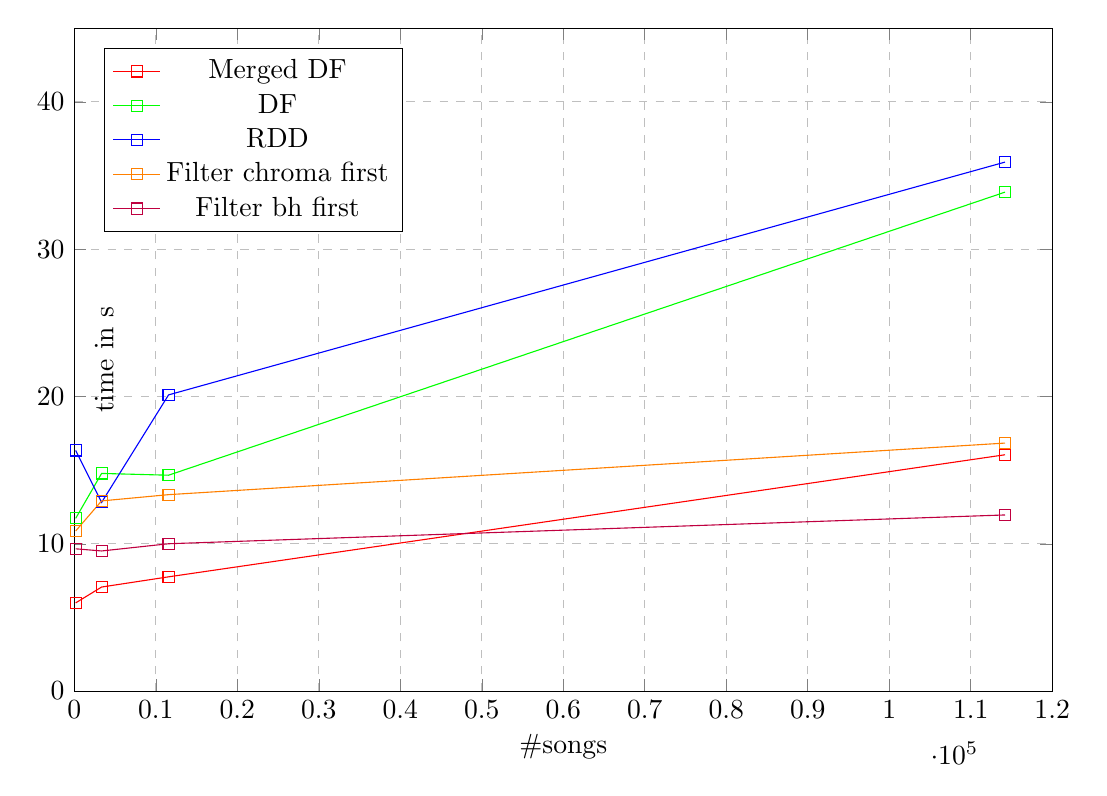
\begin{tikzpicture}
   	\centering
   	\begin{axis}[
	    x label style={at={(axis description cs:0.5,-0.05)},anchor=north},
   		y label style={at={(axis description cs:0.05,.5)},rotate=0,anchor=south},
	    xlabel={\#songs},
	    ylabel={time in s},
	    xmin=0, xmax=120000,
	    ymin=0, ymax=45,
	    legend pos=north west,
	    ymajorgrids=true,
	    grid style=dashed,
	    height=10cm,
	    width=14cm,
	    grid=major,
   	]
   	%\addplot[color=red, mark=x,]
   	%	coordinates {(164,43.090)(3344,58.852)(11564,55.227)(114210,102.438)};
   	%	\addlegendentry{Merged DF total}
   	%\addplot[color=green, mark=x,]
   	%	coordinates {(164,49.274)(3344,59.691)(11564,65.949)(114210,94.464)};
   	%	\addlegendentry{Filter total}   		
   	\addplot[color=red, mark=square, ]
   		coordinates {(164,5.987)(3344,7.063)(11564,7.756)(114210,16.043)};
   		\addlegendentry{Merged DF}
  	\addplot[color=green, mark=square,]
  		coordinates {(164,11.726)(3344,14.776)(11564,14.655)(114210,33.872)};
  	   	\addlegendentry{DF}   		
  	\addplot[color=blue, mark=square,]
  		coordinates {(164,16.337)(3344,12.809)(11564,20.108)(114210,35.911)};
  		\addlegendentry{RDD}      		
   	\addplot[color=orange, mark=square,]
   		coordinates {(164,10.870)(3344,12.910)(11564,13.335)(114210,16.836)};
   		\addlegendentry{Filter chroma first}   
   	\addplot[color=purple, mark=square,]
   		coordinates {(164,9.658)(3344,9.512)(11564,10.002)(114210,11.957)};
   		\addlegendentry{Filter bh first}   					
   	\end{axis}
   	\end{tikzpicture}
   	\caption{Descending importance filter and refine, all features}
   	\label{perfspark5}
\end{figure}
\FloatBarrier

\noindent The order of filtering for the plot labeled with "Filter chroma first" is:\\
chroma $\rightarrow$ mfcc  $\rightarrow$ js  $\rightarrow$ skl $\rightarrow$ rp  $\rightarrow$ rh  $\rightarrow$ bh  $\rightarrow$ notes\\ 
and:\\
bh $\rightarrow$ rh $\rightarrow$ notes $\rightarrow$ rp $\rightarrow$ mfcc $\rightarrow$ js $\rightarrow$ skl $\rightarrow$ chroma\\
for the plot labeled with "Filter bh first". 
\noindent The order of the different filter and refine operations is very important. For example when searching for cover songs, the cross-correlation and the levenshtein distance should be calculated in the very beginning of the filter chain or otherwise the covers songs could be filtered out. When running a simple test with the song "Für Elise" by Beethoven that appears three times in the full dataset the filter and refine method starting with the chroma features was able to still detect one alternative recording as the top recommendation and the other recording was placed as recommendation number 14, even scoring higher than in a test without the filter and refine method because other non-matching songs got filtered out.\\
Of course the computation of the cross-correlation between the chroma features is the most compute-intensive one so for performance reasons it is better to start with a distance measurement like the euclidean distance of the beat histograms because later when the more demanding computations follow the data set is already thinned out. 
This is also the reason this approach is called descending importance filter and refine in this thesis, because the client requesting song recommendations has to define which aspect is most important to him (speed, melodic/ rhythm/ timbral features or cover song detection) before choosing an order for the filter chain. The results get better the further it gets in the filter chain.  

\subsection{possible improvements and additions}

Spark offers some other interesting alternatives to compute similarities that are only mentioned here and not further evaluated.  
The Alternating Least Squares to perform collaborative filtering (see section \ref{collaborative}) would be an interesting addition. Although this thesis only focuses on audio features, a future additional implementation of metadata and listening behavior information could provide valuable informations.\\ 
The so called "DIMSUM all-pairs similarity" (Dimension Independent Similarity Computation using MapReduce) is a MapReduce algorithm to compute full similarity matrices (all-pairs similarity instead of the "one-to-many-items similarity" implemented here) and could be of interest as well.\\
Also an implementation of the TF-IDF weights is already part of the Spark framework, possibly enabling a future implementation of the melodic similarity computation using the mentioned approach in chapter \ref{textretr}
